% !TEX TS-program = XeLaTeX
% use the following command: 
% all document files must be coded in UTF-8
\documentclass{textolivre}
% for anonymous submission
%\documentclass[anonymous]{textolivre}
% to create HTML use 
%\documentclass{textolivre-html}
% See more information on the repository: https://github.com/leolca/textolivre

% Metadata
\begin{filecontents*}[overwrite]{article.xmpdata}
    \Title{El impacto del estado de alarma decretado por la COVID-19 en la inclusión educativa}
    \Author{María Pilar Cáceres Reche \sep José Antonio Marín Marín \sep Magdalena Ramos Navas-Parejo \sep Blanca Berral Ortiz}
    \Language{es}
    \Keywords{educación \sep TIC \sep COVID-19 \sep brecha digital \sep inclusión educativa \sep estudiantes en riesgo}
    \Journaltitle{Texto Livre}
    \Journalnumber{1983-3652}
    \Volume{14}
    \Issue{2}
    \Firstpage{1}
    \Lastpage{11}
    \Doi{10.35699/1983-3652.2021.34204}

    \setRGBcolorprofile{sRGB_IEC61966-2-1_black_scaled.icc}
            {sRGB_IEC61966-2-1_black_scaled}
            {sRGB IEC61966 v2.1 with black scaling}
            {http://www.color.org}
\end{filecontents*}

% used to create dummy text for the template file
\definecolor{dark-gray}{gray}{0.35} % color used to display dummy texts
\usepackage{lipsum}
\SetLipsumParListSurrounders{\colorlet{oldcolor}{.}\color{dark-gray}}{\color{oldcolor}}

% used here only to provide the XeLaTeX and BibTeX logos
\usepackage{hologo}

% used in this example to provide source code environment
%\crefname{lstlisting}{lista}{listas}
%\Crefname{lstlisting}{Lista}{Listas}
%\usepackage{listings}
%\renewcommand\lstlistingname{Lista}
%\lstset{language=bash,
        breaklines=true,
        basicstyle=\linespread{1}\small\ttfamily,
        numbers=none,xleftmargin=0.5cm,
        frame=none,
        framexleftmargin=0.5em,
        framexrightmargin=0.5em,
        showstringspaces=false,
        upquote=true,
        commentstyle=\color{gray},
        literate=%
           {á}{{\'a}}1 {é}{{\'e}}1 {í}{{\'i}}1 {ó}{{\'o}}1 {ú}{{\'u}}1 
           {à}{{\`a}}1 {è}{{\`e}}1 {ì}{{\`i}}1 {ò}{{\`o}}1 {ù}{{\`u}}1
           {ã}{{\~a}}1 {ẽ}{{\~e}}1 {ĩ}{{\~i}}1 {õ}{{\~o}}1 {ũ}{{\~u}}1
           {â}{{\^a}}1 {ê}{{\^e}}1 {î}{{\^i}}1 {ô}{{\^o}}1 {û}{{\^u}}1
           {ä}{{\"a}}1 {ë}{{\"e}}1 {ï}{{\"i}}1 {ö}{{\"o}}1 {ü}{{\"u}}1
           {Á}{{\'A}}1 {É}{{\'E}}1 {Í}{{\'I}}1 {Ó}{{\'O}}1 {Ú}{{\'U}}1
           {À}{{\`A}}1 {È}{{\`E}}1 {Ì}{{\`I}}1 {Ò}{{\`O}}1 {Ù}{{\`U}}1
           {Ã}{{\~A}}1 {Ẽ}{{\~E}}1 {Ũ}{{\~u}}1 {Õ}{{\~O}}1 {Ũ}{{\~U}}1
           {Â}{{\^A}}1 {Ê}{{\^E}}1 {Î}{{\^I}}1 {Ô}{{\^O}}1 {Û}{{\^U}}1
           {Ä}{{\"A}}1 {Ë}{{\"E}}1 {Ï}{{\"I}}1 {Ö}{{\"O}}1 {Ü}{{\"U}}1
           {ç}{{\c{c}}}1 {Ç}{{\c{C}}}1
}


\journalname{Texto Livre}
\thevolume{14}
\thenumber{2}
\theyear{2021}
\receiveddate{\DTMdisplaydate{2020}{12}{11}{-1}} % YYYY MM DD
\accepteddate{\DTMdisplaydate{2021}{02}{28}{-1}}
\publisheddate{\today}
% Corresponding author
\corrauthor{Magdalena Ramos Navas-Parejo}
% DOI
\articledoi{10.35699/1983-3652.2021.34204}
% list of available sesscions in the journal: articles, dossier, reports, essays, reviews, interviews, editorial
\articlesessionname{dossier}
%\articleid{NNNN} % if the article ID is not the last 5 numbers of its DOI, provide it using \articleid{} commmand
% Abbreviated author list for the running footer
\runningauthor{Cáceres Reche et al.}
\editorname{Anna Izabella M. Pereira}

\title{El impacto del estado de alarma decretado por la COVID-19 en la inclusión educativa}
\othertitle{O impacto do estado de alarme decretado pela COVID-19 na inclusão educacional}
\othertitle{The impact of the state of alarm decreed by COVID-19 on educational inclusion}
% if there is a third language title, add here:
%\othertitle{Artikelvorlage zur Einreichung beim Texto Livre Journal}

\author[1]{María Pilar Cáceres Reche \orcid{0000-0002-6323-8054} \thanks{Email: \url{caceres@ugr.es}}}
\author[1]{José Antonio Marín Marín \orcid{0000-0001-8623-4796} \thanks{Email: \url{jmarin@ugr.es}}}
\author[1]{Magdalena Ramos Navas-Parejo \orcid{0000-0001-9477-6325} \thanks{Email: \url{magdalena@ugr.es}}}
\author[1]{Blanca Berral Ortiz \orcid{0000-0001-8139-8468} \thanks{Email: \url{blancaberral@correo.ugr.es}}}

\affil[1]{Universidad de Granada, Facultad de Ciencias de la Educación, Departamento de Didáctica y Organización Escolar, Granada, España.}

\addbibresource{article.bib}
% use biber instead of bibtex
% $ biber tl-article-template

% set language of the article
\setdefaultlanguage{spanish}
\setotherlanguage{portuguese}
\setotherlanguage{english}

% for spanish, use:
%\setdefaultlanguage{spanish}
\gappto\captionsspanish{\renewcommand{\tablename}{Tabla}} % use 'Tabla' instead of 'Cuadro'
\AfterEndPreamble{\crefname{table}{tabla}{tablas}\Crefname{table}{Tabla}{Tablas}}

% for languages that use special fonts, you must provide the typeface that will be used
% \setotherlanguage{arabic}
% \newfontfamily\arabicfont[Script=Arabic]{Amiri}
% \newfontfamily\arabicfontsf[Script=Arabic]{Amiri}
% \newfontfamily\arabicfonttt[Script=Arabic]{Amiri}
%
% in the article, to add arabic text use: \textlang{arabic}{ ... }

% to use emoticons in your manuscript
% https://stackoverflow.com/questions/190145/how-to-insert-emoticons-in-latex/57076064
% using font Symbola, which has full support
% the font may be downloaded at:
% https://dn-works.com/ufas/
% add to preamble:
% \newfontfamily\Symbola{Symbola}
% in the text use:
% {\Symbola }

% reference itens in a descriptive list using their labels instead of numbers
% insert the code below in the preambule:
\makeatletter
\let\orgdescriptionlabel\descriptionlabel
\renewcommand*{\descriptionlabel}[1]{%
  \let\orglabel\label
  \let\label\@gobble
  \phantomsection
  \edef\@currentlabel{#1\unskip}%
  \let\label\orglabel
  \orgdescriptionlabel{#1}%
}
\makeatother
%
% in your document, use as illustraded here:
%\begin{description}
%  \item[first\label{itm1}] this is only an example;
%  % ...  add more items
%\end{description}
 

% custom epigraph - BEGIN 
%%% https://tex.stackexchange.com/questions/193178/specific-epigraph-style
\usepackage{epigraph}
\renewcommand\textflush{flushright}
\makeatletter
\newlength\epitextskip
\pretocmd{\@epitext}{\em}{}{}
\apptocmd{\@epitext}{\em}{}{}
\patchcmd{\epigraph}{\@epitext{#1}\\}{\@epitext{#1}\\[\epitextskip]}{}{}
\makeatother
\setlength\epigraphrule{0pt}
\setlength\epitextskip{0.5ex}
\setlength\epigraphwidth{.7\textwidth}
% custom epigraph - END


% if you use multirows in a table, include the multirow package
\usepackage{multirow}

% add line numbers for submission
%\usepackage{lineno}
%\linenumbers

\begin{document}
\maketitle

\begin{polyabstract}
\begin{abstract}
El estado de alarma decretado en la mayoría de los países, a causa de la COVID-19, obligó a cerrar las escuelas. Lo que supuso un cambio abrupto en la forma de enseñanza para el que muchos de los docentes, familias y alumnado no estaban preparados. Las TIC adquirieron un especial protagonismo, ya que se convirtieron en la única vía para acceder a la educación. Esta situación ha llegado en un momento en el que las diferencias socioeconómicas mantienen una brecha digital abierta que impide que se pueda hablar de igualdad de oportunidades en educación y por tanto de inclusión educativa. El objetivo de este trabajo ha sido realizar una revisión bibliográfica para poder determinar las consecuencias que este cambio radical de enseñanza ha tenido en el proceso de inclusión educativa, cómo ha afectado a la población más vulnerable y a los docentes y qué ha supuesto para la conocida brecha digital. Para ello, se ha accedido a los distintos artículos publicados sobre este ámbito en el último año en diferentes bases de datos que hacen referencia a la inclusión educativa. Las conclusiones más relevantes parten de la evidencia de la importancia de cerrar esta brecha digital que ha dejado sin acceso a la educación a millones de estudiantes en todo el mundo y del gran avance que se ha obtenido en cuestiones de experiencia y formación de la comunidad educativa en general, en TIC y metodologías activas y autónomas para el aprendizaje del alumnado.

\keywords{educación \sep TIC \sep COVID-19 \sep brecha digital \sep inclusión educativa \sep estudiantes en riesgo}
\end{abstract}

\begin{portuguese}
\begin{abstract}
O estado de alarme decretado na maioria dos países, devido ao COVID-19, obrigou as escolas a fechar. Isto significou uma mudança abrupta na forma de ensinar para a qual muitos professores, famílias e estudantes não estavam preparados. As TIC assumiram um papel especial uma vez que se tornou a única forma de acesso à educação. Esta situação chegou numa altura em que as diferenças socioeconómicas mantêm uma fractura digital aberta que nos impede de falar de igualdade de oportunidades na educação e, por conseguinte, de inclusão educacional. O objectivo deste trabalho foi realizar uma revisão bibliográfica a fim de determinar as consequências que esta mudança radical no ensino tem tido no processo de inclusão educacional, como tem afectado a população e os professores mais vulneráveis e o que tem significado para a chamada fractura digital. Para o efeito, acedemos aos diferentes artigos publicados neste campo no último ano em diferentes bases de dados que se referem à inclusão educacional. As conclusões mais relevantes baseiam-se na evidência da importância de eliminar esta fractura digital que tem deixado milhões de estudantes em todo o mundo sem acesso à educação e no grande progresso que tem sido obtido, em termos de experiência e formação da comunidade educativa em geral, nas TIC e nas metodologias activas e autónomas de aprendizagem dos estudantes.

\keywords{educação \sep TIC \sep COVID-19 \sep divisão digital \sep inclusão educacional \sep estudantes em risco}
\end{abstract}
\end{portuguese}

\begin{english}
\begin{abstract}
The state of alarm decreed in most countries, due to Covid-19, forced schools to close. This meant an abrupt change in the way of teaching for which many of the teachers, families and students were unprepared. ITC took on a special role as they became the only way to access education. This situation came at a time when socio-economic differences maintained an open digital divide that prevents us from talking about equal opportunities in education and therefore educational inclusion. The aim of this study was to carry out a literature review in order to determine the consequences that this radical change in teaching has had on the process of educational inclusion, how it has affected the most vulnerable population and teachers, and what it has meant for the so-called digital divide. To this end, access has been gained to the different articles published on this field in the last year in different databases that refer to educational inclusion. The most relevant conclusions are based on the evidence of the importance of closing this digital divide that has left millions of students around the world without access to education and the great progress that has been made, in terms of experience and training of the educational community in general, in ITC and more active and autonomous methodologies for students.

\keywords{education \sep ITC \sep COVID-19 \sep digital divide \sep educational inclusion \sep at risk student}
\end{abstract}
\end{english}

% if there is another abstract, insert it here using the same scheme
\end{polyabstract}


\section{Introducción}\label{sec-intro}
La COVID-19 se propagó rápidamente por todo el mundo causando una crisis sanitaria tal, que los gobiernos se vieron en la obligación de decretar el estado de alarma en la mayoría de los países. Para evitar el contagio masivo del virus, los ciudadanos pasaron varios meses en sus casas en cuarentena, rompiendo con cualquier actividad cotidiana llevada a cabo hasta el momento. Por este motivo, para que el alumnado pudiera continuar con su formación educativa, no quedó otra alternativa que utilizar los espacios virtuales. Lo que generó la implantación urgente de una enseñanza a distancia, en la que se hacía necesario contar con la formación adecuada para el manejo de las Tecnologías de la Información y la Comunicación (TIC), estar en posesión de dispositivos tecnológicos, disponer de conexión a internet y tener conocimiento sobre las metodologías didácticas online \cite{rojaslondono2020}.

Si se tiene en cuenta que, según \textcite{globaldigital2020}, el 60\% de la población mundial tiene acceso a internet, significa que el otro 40\% de la población queda excluido de esta forma de enseñanza, quedándose sin poder acceder a la educación, que le pertenece por derecho, durante los meses que ha durado el estado de alarma. La brecha digital se hace más evidente que nunca, junto con la certeza de que, aunque estamos en proceso, nos encontramos lejos de llegar a una inclusión educativa que garantice la igualdad de oportunidades y la calidad educativa de todo el alumnado sin excepción.

En esta revisión bibliográfica se ha planteado como objetivo determinar las consecuencias que esta nueva forma de enseñanza, que ha venido impuesta para preservar la salud de los ciudadanos, ha tenido en el proceso de inclusión educativa. Las preguntas de investigación son las siguientes: ¿cómo ha afectado el estado de alarma en la educación de la población más vulnerable?, ¿qué ha supuesto para la conocida brecha digital? y ¿qué aspectos positivos se pueden desprender de esta vivencia para la educación?

\section{La inclusión educativa}
La educación del siglo XXI se ha encontrado con el reto de cumplir con el principio de igualdad, debido a la llegada de dos nuevos fenómenos: el de la globalización y el postmodernismo, los cuales ponen a prueba la igualdad de oportunidades en educación \cite{garciapedraza2015}.

Según \textcite{reales2005} no cabe duda de que la educación actúa como agente de cambio social. Nos encontramos en constante evolución, pero estos cambios no se producen de forma uniforme ni predecible, por lo que no se pueden esperar transformaciones coherentes ni únicas. Dentro de este panorama, la escuela puede influir de manera positiva y constructiva en las condiciones sociales.

En la sociedad global en la que vivimos actualmente, la educación exige a los docentes y a la ciudadanía en general, el replanteamiento de las prácticas educativas, para otorgarles  un enfoque nuevo, que respete la diversidad, en cualquiera de sus dimensiones, y que luche contra cualquier tipo de desigualdad y exclusión \cite{carmona-santiago2019}. La escuela debe adquirir este papel de agente que impulse la transformación social, desde la participación comunitaria y democrática, utilizando como ejes fundamentales la inclusión, la interculturalidad, la democratización y la territorialización \cite{salesciges2019}.

El término inclusión se entiende desde distintas perspectivas, que \textcite{caberoalmenara2017} encuadran en las que se observan en la \Cref{fig1}:

\begin{figure}[htbp]
 \centering
 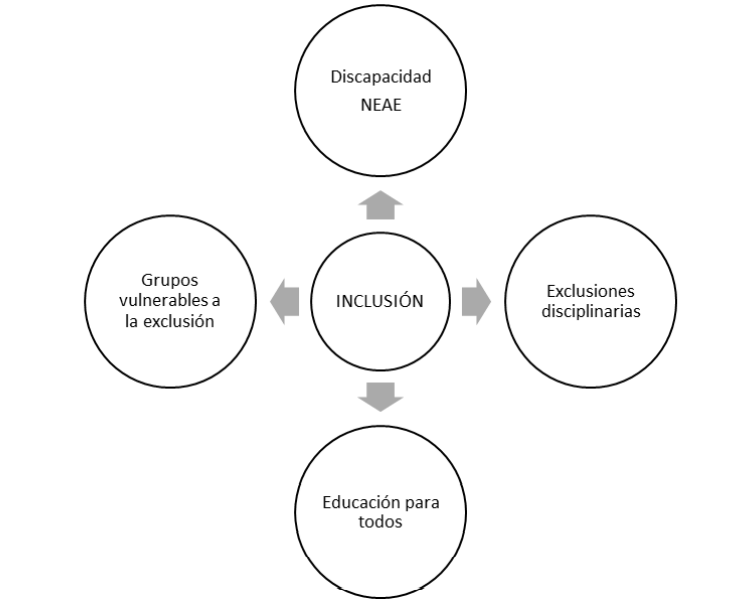
\includegraphics[width=0.75\textwidth]{imagem1.png}
 \caption{Perspectivas del término inclusión.}
 \label{fig1}
 \source{elaboración propia a partir de \textcite{caberoalmenara2017}.}
\end{figure}

La inclusión, desde la perspectiva de estos autores, se concibe como una educación global, que pone el foco en la igualdad y el dominio colectivo. Se trata de  una educación para todos, que atiende al derecho que tienen todas las personas, sin ningún tipo de excepción, a la educación y que incorpora a esos colectivos que, tradicionalmente, se han encontrado excluidos por razones de género, cultura, raza o características personales.

La inclusión es una evolución del término integración, que no solo se refiere al individuo, se centra también en el aula, examinando los factores de enseñanza-aprendizaje, resolviendo las dificultades en colaboración con otros profesionales, estableciendo estrategias docentes, facilitando un entorno de adaptación y ofreciendo estructuras organizativas que flexibilicen la incorporación de la persona. Se pasa así de un modelo individual, donde la dificultad reside únicamente en el alumnado, a un modelo social, en el que las dificultades y limitaciones se encuentran en la sociedad \cite{gallegoortega2016}.

La educación inclusiva debe entenderse como un proceso cuya base reside en un cambio de paradigma ideológico con unos planteamientos de intervención sustentados a su vez por valores de derecho, calidad y equidad, los cuales deben compartir los políticos, docentes, las familias y la sociedad en general \cite{muntaner2019}.

\subsection{El papel de las TIC en la inclusión educativa}
Una de las características fundamentales de la sociedad de hoy día reside en la importancia que tienen en ella las TIC. Por este motivo ha pasado a llamarse la sociedad digital o sociedad de la información, debido al cúmulo de información que se produce con la aceleración de las interacciones y dinámicas sociales, propiciadas por el avance de  la tecnología \cite{hernandez2017, cabero-almenara2019}.

La educación también se ha visto fuertemente influenciada por la tecnología, transformando las formas de interacción, comunicación, estudio e investigación, convirtiéndose en el eje central de las oportunidades de innovación educativa y desarrollo. Esta incorporación de las TIC se ha ido realizando a través de un proceso que ha supuesto, además del uso de estos dispositivos tecnológicos que sustituyen a los tradicionales (pizarras digitales, tablets, etc.), la construcción de nuevas formas pedagógicas y la consolidación de un aprendizaje significativo y autónomo basado en ellas \cite{caceresreche2020}. Hoy día, las TIC son herramientas educativas que tienen la capacidad de mejorar la calidad de la educación, revolucionando la forma en la que se accede y se interpreta la información \cite{morenoguerrero2020}.

Según \textcite{fernandezbatanero2019}, estas poseen un alto nivel igualador de oportunidades, dado el papel que ejercen como facilitadoras de la comunicación e interacción de todo el alumnado, sean cual sean sus limitaciones. Si se utilizan con la metodología didáctica adecuada, pueden romper con las barreras del espacio y el tiempo, permitiendo la participación y el aprendizaje descontextualizado y ubicuo, pueden fomentar el trabajo colaborativo, el aprendizaje independiente y el autoaprendizaje, la integración social y la autonomía, aspectos fundamentales para la inclusión del alumnado \cite{cascales-martinez2018}. A través de las TIC se pueden ofrecer posibilidades de comunicación interactiva, tratamiento de imágenes, simulaciones de experimentos o fenómenos, construcción de modelos y analogías, resolución de problemas, acceso a la información y manejo de todo tipo de datos \cite{cadenagonzalez2019}. Además de mejorar la motivación y actitud del alumnado, siempre y cuando sigan una estructura didáctica acorde a las necesidades de aprendizaje de los discentes \cite{morenoguerrero2018}.  

\textcite{caberoalmenara2017} definen la relación de las TIC y la inclusión educativa desde una doble perspectiva: 1) la que se refiere al uso de la tecnología para favorecer una educación de calidad, tras la eliminación de las barreras que impiden la participación de toda la diversidad del alumnado, 2) la que por medio de la planificación tecnológica permite entornos accesibles que facilitan la inclusión, reduciendo la llamada brecha digital. La cual se entiende como la diferenciación entre el alumnado que tiene acceso a loa medios digitales y a internet y el que no, lo que propicia situaciones de desigualdad de oportunidades.

La tecnología, en vista de lo expuesto, representa un papel importante en la inclusión educativa. Además, se puede encontrar dentro de los elementos fundamentales con los que debe contar una escuela inclusiva (\Cref{fig2}), según \textcite{caberoalmenara2017}.

\begin{figure}[htbp]
 \centering
 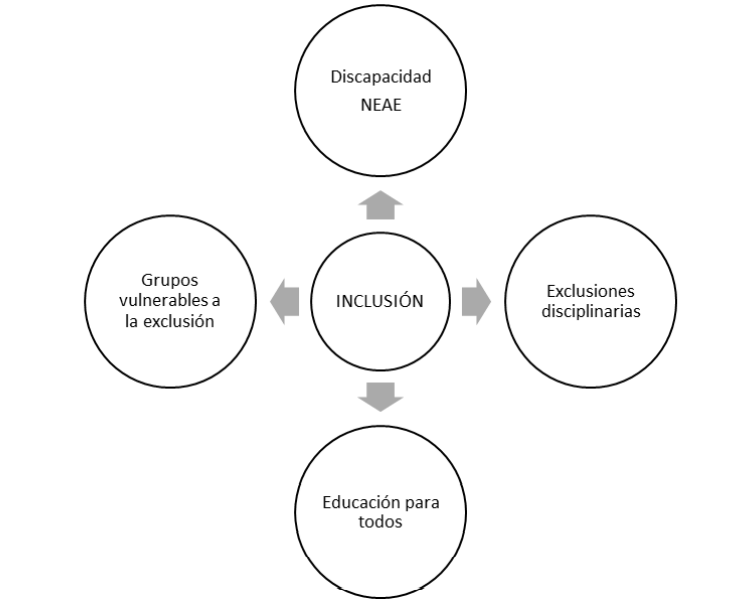
\includegraphics[width=0.85\textwidth]{imagem2.png}
 \caption{Elementos que componen una escuela inclusiva.}
 \label{fig2}
 \source{elaboración propia a partir de \textcite{caberoalmenara2017}.}
\end{figure}

Por tanto, la búsqueda de respuestas a la diversidad de las aulas supone el punto de partida de la educación inclusiva del siglo XXI, a partir del cual entrar en el complejo proceso de conseguir una educación para todos igual, acercando los procesos de enseñanza a la diversidad de alumnado que se encuentra en las aulas. Las TIC suponen un gran aliado dentro de este proceso, las cuales deben ir ligadas a una adecuada formación del profesorado en competencias digitales e inclusivas, además de ser accesibles para que puedan llegar a todos sin excepción e ir acompañadas de la metodología más idónea \cite{marindiaz2020}.

\subsection{La brecha digital}
La fuerte evolución de los medios de comunicación de los últimos años ha dejado en evidencia el gran potencial de desarrollo económico, social y cultural que aportan las TIC. Sin embargo, este desarrollo no se ha percibido de la misma forma en todos los territorios, ni en los mismos niveles socioeconómicos, ya que dependen de muchas variables.

La inexistencia de igualdad de oportunidades de muchos escolares, debida a distintos factores, hace que resulte muy complicado disponer de estos recursos y, por tanto, ofrecer una educación de calidad que dé respuesta a las exigencias del siglo XXI \cite{moralesromo2017}.

Las barreras que separan a los individuos de las TIC pueden ser de diferentes índoles, que van desde la falta de competencias necesarias para su efectiva utilización, hasta la falta de acceso a los recursos digitales y/o conexión, debido a las bajas rentas o a una situación de aislamiento. Estas circunstancias son las que generan esta situación de desigualdad que, a su vez, supone entrar en un proceso de exclusión social. Lo que se evidencia hoy día más que nunca, dada la importancia que han adquirido las TIC en todas dimensiones del desarrollo humano \cite{martinezlopez2020}.

La tecnología, por tanto, puede ser un elemento inclusivo pero también de discriminación y exclusión en algunas circunstancias y en determinados contextos sociales si no se puede contar con ella. Para tratar de paliar esta realidad, las distintas instituciones han desarrollado planes formativos y han realizado importantes inversiones para fomentar su uso. Pero hoy día, aún nos encontramos muy lejos de llegar a unos resultados óptimos \cite{caberoalmenara2017}.

La brecha digital supone el reflejo de las desigualdades sociales dentro de un mundo  movido por la tecnología \textcite{caberoalmenara2017} la definen como la diferenciación producida entre aquellas personas, instituciones, sociedades o países que tienen la posibilidad de acceder a las TIC de forma general y a internet y las que no. Se define en términos de desigualdad de oportunidades para acceder a la información, el conocimiento y la educación mediante la tecnología, por motivos económicos, de edad, género, raza, ubicación geográfica y formación entre otros. En palabras de \textcite{cervantesholguin2020} nos encontramos en riesgo de que la brecha digital se convierta en una brecha de aprendizaje debido a la importancia que han adquirido las TIC en el ámbito educativo.

En el caso concreto de España, la brecha digital se asocia con las situaciones de pobreza y exclusión social. Esta realidad tardó mucho en ser reconocida por los poderes públicos. Fue en 2013 cuando el Estado asumió que debía considerarse como parte de las situaciones de vulnerabilidad que se producen en el país, por lo que creó el Plan Nacional de Acción para la Inclusión social 2013-2016 (PNAIS). Este documento plasma los riesgos de la sociedad de la información y su influencia en la desigualdad de oportunidades de desarrollo profesional, personal y social, considerándola un factor de riesgo de exclusión social \cite{rodiciogarcia2020}.

En España el género ya no supone una variable que se asocie con el acceso a la tecnología. Los estudios realizados concluyeron en 2019 afirmando que no existían desigualdades en el uso de internet entre hombres y mujeres, incluso las mujeres superaban a los hombres en el uso diario, según los resultados del Instituto Nacional de Estadística (INE) de este mismo año. Sin embargo, variables como la edad o el nivel educativo de las familias sí se asocian directamente con el acceso a las TIC \cite{acosta2020}.

En Madrid, por ejemplo, según los datos recogidos por el INE en 2019 a través de una encuesta sobre equipamiento y uso de TIC en los hogares, se obtuvo como resultado que el 1,3\% de las viviendas donde reside una persona menor de 16 años al menos, no dispone de conexión a internet e incluso el 2,8\% no cuenta con ordenador. Estas cifras suponen más de 600.000 hogares en la Comunidad de Madrid \cite{martinezlopez2020}.

\section{La importancia de las TIC durante el estado de alarma en la educación}
Las medidas que el gobierno español se vio obligado a tomar en el Real Decreto, por el que se declaró el estado de alarma, para vencer la pandemia mundial producida por la COVID-19, impactaron de manera directa en la educación, afectando a todo el alumnado de todos los niveles educativos. La suspensión de la actividad docente presencial de manera abrupta, supuso el ralentizamiento de los aprendizajes de la población escolar en general, pero en el caso de los entornos más vulnerables, se paralizó, no solo el aprendizaje, si no la protección y la posibilidad de alcanzar mejores condiciones de vida. Puesto que la escuela se considera la mejor herramienta de compensación de las desigualdades sociales \cite{espinosa2020}.

Internet ha resultado ser la única solución para poder unir a las familias y amigos, para continuar con la actividad educativa, atención médica, asesorías legales, revisorías fiscales y estructurales y en general para mantener la conectividad ya sea de servicios, laboral, educativa o social, durante el confinamiento total que se ha vivido en la mayoría de los países a causa de la pandemia de la COVID-19 \cite{lopezdaza2020}.

Para el 20 de abril de 2020, el impacto del cierre de los centros educativos se estimó en el 91,3\% (1.575.270.054) de la población estudiantil mundial. Donde la única manera de continuar con la educación era a través del uso de las TIC. Pero como se ha comentado anteriormente, antes de que se dieran estas circunstancias, ya existía una pronunciada brecha digital que afecta a los sectores más desfavorecidos de la población, que no cuentan ni con dispositivos tecnológicos, ni tienen la formación adecuada para manejarlos, ni conectividad \cite{lopezdaza2020}.

Desde la Organización de las Naciones Unidas (ONU), el Secretario General Guterres solicitó en un informe, el 16 de abril de 2020, que los gobiernos invirtieran en recursos suficientes para adoptar medidas que paliaran los efectos que estaba produciendo la pandemia en la infancia más vulnerable. Puesto que la estaba llevando a la pobreza, impidiendo su aprendizaje, amenazando su supervivencia y salud \cite{onu2020}.

Por tanto, esta situación de desamparo educativo, causado por la paralización de las clases presenciales, afectó especialmente a la población desfavorecida socialmente. Coincidiendo con los que ya se encontraban excluidos a causa de la brecha digital, que se ha hecho mucho más evidente y ancha con la situación de estado de alarma que han sufrido la mayoría de los países a nivel mundial. Los territorios donde la situación de desigualdad ya era grave, como los que se encuentran en América Latina, en los que ya existe una diferencia muy pronunciada entre el rendimiento académico en función del estrato social de pertenencia, la pandemia ha dejado completamente excluida a su población más vulnerable \cite{alvarez-gardyn2020, barbozacid2020}. En Latinoamérica, solo 4 de cada 10 hogares cuenta con conexión internet y, además, el profesorado con competencias digitales para utilizar las TIC de forma pedagógica en entornos virtuales, supone una minoría \cite{murillo2020}.

Además de la interrupción del aprendizaje, los padres de estas familias en riesgo de exclusión social, aparte de no poseer acceso a las plataformas digitales, no suelen contar con la preparación adecuada para realizar una enseñanza a distancia. Esta situación ha ocasionado que las tasas de abandono escolar se hayan incrementado en el último año considerablemente \cite{murillo2020}.

Ha quedado evidente la importancia que suponen las TIC, por la facilidad de acceso que han aportado a todos los niveles, así como las desigualdades que genera la falta de estos recursos en la población. La comunicación y la conectividad no se pueden entender por separado. Internet posee un papel principal en el desarrollo social, por lo que se debe concebir como un derecho por su carácter fundamental y así lo ha subrayado esta situación generada por la COVID-19, que ha mermado el derecho a la educación de muchos niños y a la igualdad de oportunidades \cite{martinezlopez2020}.

\subsection{Los docentes y las TIC durante el estado de alarma}
Antes de que los docentes se encontraran con el estado de alarma sin aviso previo y sin otra posibilidad de realizar su labor educativa que no fuera a través de plataformas digitales, existía aún un alto porcentaje que se resistía a redefinir sus roles tradicionales e incluir metodologías activas y TIC en sus procesos de enseñanza-aprendizaje. Pese a la importancia de realizar este cambio metodológico, que da un alto protagonismo a las TIC, no se había conseguido una integración adecuada en los procesos de formación del profesorado \cite{rodriguezgarcia2018}. Ni siquiera con su aumento, las inversiones realizadas y el interés por la formación del profesorado con la puesta en marcha de planes específicos, se había conseguido transformar completamente la práctica educativa para crear nuevos escenarios de comunicación entre los agentes que componen la comunidad educativa \cite{caberoalmenara2017}.

Tampoco las administraciones han realizado la inversión necesaria para generar entornos virtuales con la calidad suficiente para que se pueda llevar a cabo un curso escolar de forma telemática. Este hecho ha supuesto que los docentes hayan tenido que improvisar y desarrollar procesos de cambio que se encontraban en una fase muy incipiente en muchos casos. De esta forma, las resistencias a las TIC se han visto superadas por la obligación de emplearlas \cite{martinezlopez2020}.

\subsection{Efectos positivos del aislamiento social en la educación}
La situación de aislamiento ha supuesto un reto educativo y una oportunidad para que el alumnado investigue y construya su propio conocimiento \cite{ceballosmaron2020} y para que los docentes se vean en la obligación de adoptar a las TIC como aliadas del proceso de enseñanza-aprendizaje, conociendo nuevas herramientas y espacios educativos más allá de los tradicionales.

Los sistemas educativos han tenido que abandonar su modelo pedagógico tradicional y presencial, por otro muy distinto, en el cual el aprendizaje se desarrolla de forma digital y tiene lugar en entornos virtuales, lo que ha supuesto un desafío para toda la comunidad educativa, por la forma tan abrupta de llevarlo a cabo. A día de hoy, han adquirido mucha fuerza los entornos virtuales de aprendizaje tales como E-learning, M-learning, B-learning. Se ha dado un paso muy grande en el proceso de integración de las TIC y los modelos pedagógicos virtuales en muy poco tiempo. Resulta evidente el hecho de que se puede educar de una manera diferente contando con los medios adecuados \cite{moraaristega2021}. Pasada esta situación de emergencia, alumnado y profesorado habrán aumentado sus competencias digitales de forma considerable. Pero para que este modelo digital tenga éxito en la totalidad del alumnado sin exclusión, hace falta implementar los recursos tecnológicos necesarios, tanto dispositivos como conexión, la capacitación de los docentes y la adaptación del alumnado a la nueva forma de educación, ofreciendo siempre una educación de calidad \cite{condor-herrera2020}.

Las familias, como parte importante de la comunidad educativa, se han visto en la obligación de colaborar en las actividades didácticas de sus hijos, desarrollando la empatía hacia el aprendizaje de los mismos, lo que ha supuesto un aspecto positivo para el desarrollo de la educación del alumnado \cite{moraaristega2021}.

Otro aspecto positivo que ha surgido con el paso de la COVID-19 por el mundo, ha sido la toma de conciencia por luchar contra la brecha digital para erradicar las desigualdades que llevan a que cada día más estudiantes abandonen sus estudios. Esta crisis ha generado la necesidad de fomentar medidas urgentes para conseguir la inclusión educativa que contrarreste las desigualdades sociales \cite{rojaslondono2020}.

La necesidad de incorporar herramientas tecnológicas en educación y la comprobación de su efectividad, ha conllevado a valorar sus potencialidades y al análisis de metodologías interactivas que aumentan la calidad educativa y dan una mejor respuesta a la educación de la sociedad del siglo XXI en la que nos encontramos. Como ejemplo, el modelo de enseñanza Flipped Classroom o clase invertida hace años que se considera una metodología educativa que mejora los aprendizajes del alumnado a través del autoaprendizaje y el desarrollo de capacidades de investigación, observación, reflexión, análisis, interpretación y síntesis de sus propios conocimientos \cite{rodriguez+hidalgo2018, carreno2019}. Sin embargo, todavía no se encontraba muy extendido. Ahora, que el alumnado ha aprendido a responsabilizarse y gestionar su conocimiento de forma autónoma y que el profesorado ha dado un gran paso en sus competencias y conocimiento sobre TIC y metodologías activas, resultará más fácil su implantación, pudiendo hacer uso de sus ventajas y potencialidades. 

Diferentes estudios, como el llevado a cabo por \textcite{ardini2020}, muestran las herramientas TIC más utilizadas por los docentes durante la pandemia; el 67,6\% de los docentes ha integrado el uso de Whatsapp en sus aulas y han empleado el uso de entornos virtuales como Moodle, Microsoft Teams o Edmodo. El 61,3\% ha utilizado Zoom, Google Meet o Youtube para realizar videoconferencias. Además de utilizar Facebook, murales digitales como Genial.ly, Maural.ly y evaluar a través de Kahoot y Quiziz.

\section{Discusión y conclusiones}
La calidad de un sistema educativo se mide por su capacidad de atender a todo el alumnado de la mejor manera posible. Dentro de la práctica docente se deben encontrar los términos como: normalización, inclusión, atención a la diversidad y metodologías activas y TIC.

La inclusión educativa es una de las máximas de nuestro sistema educativo, según el criterio de la UNESCO en el que intervienen el acceso, la participación y la calidad de la enseñanza. No se puede hablar de inclusión educativa sin una inclusión de las TIC previa, además de otros muchas variables que perpetúan las desigualdades y por tanto la exclusión de ciertos colectivos vulnerables. En este proceso se encuentran implicados numerosas factores: administrativos, políticos, educativos, sociales y familiares.

La pandemia generada por la COVID-19 ha demostrado que la inclusión digital y educativa son procesos inacabados que afectan negativa y directamente a los más desfavorecidos. Las TIC, ahora más que nunca, suponen un requisito fundamental para poder participar de una sociedad tecnológica. Se habrán conseguido integrar a las TIC cuando, a través de su uso y con la metodología adecuada, se consiga un aprendizaje significativo, contextualizado, autónomo y ubicuo que no excluya a ningún individuo.

Esta situación ha obligado a los docentes a formarse y experimentar con entornos virtuales, al igual que su alumnado, lo que ha supuesto un gran avance para la integración de las TIC en el ámbito educativo y un gran paso para acortar la brecha digital ocasionada por la falta de competencia digital del profesorado y los discentes.

Antes de la llegada de la COVID-19, utilizar las TIC en educación era opcional y en muchas ocasiones una herramienta más en el aula que sustituía a los recursos tradicionales, sin que supusiera una variación de la metodología. Sin embargo, tras la pandemia se ha hecho imprescindible el dominio y conocimiento del uso adecuado de las plataformas virtuales para generar un aprendizaje dinámico y significativo. Esto ha supuesto un reto para muchos docentes que han tenido que exponer sus habilidades tecnológicas y conocimientos sobre metodologías educativas y canales de comunicación a través de TIC.

Las evidencias han dado cuenta de que se puede educar de manera diferente y del camino que queda por recorrer para conseguir la inclusión de las TIC, como parte integrada en la inclusión educativa general, que elimine la brecha digital, la cual se ha puesto de claro manifiesto durante el estado de alarma en la mayoría de los países. Lo que podría ser utilizado por las administraciones educativas para la toma de decisiones de cara al futuro, reformulando las políticas para alcanzar una educación inclusiva más justa e igualitaria \cite{alvarez-gardyn2020}.Esta situación ha supuesto un gran paso para la concienciación de este problema del que ya el Secretario General de la ONU; Guterres, se ha hecho eco y ha difundido a través de un informe \cite{onu2020}.

Con la realización de este trabajo se han dado respuesta al objetivo y a las preguntas de investigación planteadas y se permite la continuación de esta línea de investigación que queda abierta para medir en un futuro el impacto que ha producido el cierre de las escuelas por la COVID-19 en los avances en la integración de las TIC en educación, el acortamiento de la brecha digital y en la inclusión educativa en general.


\printbibliography\label{sec-bib}
% if the text is not in Portuguese, it might be necessary to use the code below instead to print the correct ABNT abbreviations [s.n.], [s.l.] 
%\begin{portuguese}
%\printbibliography[title={Bibliography}]
%\end{portuguese}


\end{document}
